\documentclass[a0paper,landscape,showframe]{baposter}

%%%%lualatex on
%\usepackage{luatextra}
\usepackage{fontspec}
%Ligatures={Contextual, Common, Historical, Rare, Discretionary}
\setmainfont[Mapping=tex-text]{Linux Libertine O}

%%%lua off
%\usepackage[utf8x]{inputenc}
%\usepackage[T1]{fontenc} 
%\usepackage{lmodern}

\usepackage{enumerate}
\usepackage[english]{babel}
\usepackage{graphicx} %to insert pictures
\usepackage{color} %to set colors
\usepackage{algorithm,algorithmicx,algpseudocode}
\usepackage{mathtools}
\usepackage{latexsym}
\usepackage{caption}
\usepackage{multicol}

\usepackage{float}
\usepackage{booktabs}
\algnewcommand\And{\textbf{and}}

\DeclarePairedDelimiter\abs{\lvert}{\rvert}%
\DeclarePairedDelimiter\norm{\lVert}{\rVert}%

\newcommand{\specialcell}[2][c]{%
  \begin{tabular}[#1]{@{}c@{}}#2\end{tabular}}


\makeatletter
\let\oldabs\abs
\def\abs{\@ifstar{\oldabs}{\oldabs*}}
\let\oldnorm\norm
\def\norm{\@ifstar{\oldnorm}{\oldnorm*}}
\makeatother


%\usepackage[top=1.5cm,bottom=2cm,left=2.5cm,right=2.5cm]{geometry}
%\linespread{1.5}\selectfont



\author{Simon Carrignon}
\definecolor{bordercol}{RGB}{255,255,255}

\definecolor{headercol1}{RGB}{3,51,123}
\definecolor{bscol}{RGB}{3,51,123}
\definecolor{headercol2}{RGB}{255,255,255}
\definecolor{headerfontcol}{RGB}{255,255,255}
\definecolor{boxcolor}{RGB}{255,255,255}
\definecolor{emphcol}{RGB}{106,105,180}

%%% Save space in lists. Use this after the opening of the list %%%%%%%%%%%%%%%%
\newcommand{\compresslist}{
	\setlength{\itemsep}{1pt}
	\setlength{\parskip}{0pt}
	\setlength{\parsep}{0pt}
}
\newcommand{\coloremph}[1]{
	\textcolor{emphcol}{\bf#1}
}


\begin{document}

\begin{poster}{
	borderColor=bordercol,
	headerColorOne=headercol1,
	headerColorTwo=headercol2,
	headerFontColor=headerfontcol,
	% Only simple background color used, no shading, so boxColorTwo isn't necessary
	boxColorOne=boxcolor,
	headershape=roundedright,
	headerfont=\Large\sf\bf,
	textborder=rectangle,
	headerborder=open,
	background=plain,
	bgColorOne=white,
	boxshade=plain,
	grid,
	columns=3
}
{
Eye Catcher, empty if option eyecatcher=no
}
{
	Modelling the Co-evolution of Trade and Culture 
}
{
	Simon Carrignon,
	Jean-Marc Montanier and
	Xavier Rubio-Campillo\\
	{\small contact:simon.carrignon@bsc.es}
}
{
\setlength\fboxsep{0pt}
\setlength\fboxrule{0.5pt}
		\begin{minipage}{14em}
			%\vspace*{\stretch{1}}
			
\includegraphics[height=4em]{bscLogo.jpg}
			%\vspace*{\stretch{1}}
			%
\includegraphics[angle=90,width=2.5em]{MemoireLophiss/images/logo_p7_large}
		\end{minipage}
}

\headerbox{Introduction}{name=introduction,column=0,row=0}{
% the spread of cultural traits is often modelled following neutral theory

Cultural change comprises  processes that modify spread of information by social interaction within a population~\cite{boyd_origin_2005}. An increasing number of social scientists are using an evolutionary framework to model this~\cite{henrich_evolution_2003}.

%This approach aims at fostering the development of transdisciplinary efforts designed to understand cultural change.

%Several studies focus on the biases that affect the transmission of cultural traits, including the relevance of intrinsic traits and frequency dependence properties. These analysis often compare evidences against neutral models~\cite{neiman_stylistic_1995}.They assume that traits do not affect the fitness of the individual that acquires it; within this context its transmission is unbiased, and its success will depend on its popularity amongst the rest of individuals. This neutral model generates a distinctive pattern of frequency distribution of traits, identified as a power law. 
We use this framework to study economic activity. This phenomenon depends on particular cultural traits: the value attributed to each goods. Multiple biases could explain the fact that those value are transmitted more readily than the others. Some of those biases can be explained by the intrinsic properties of a trait (how beneficial it is), while others are simply explained by the frequency of these traits (how popular a it is). It is the impact of such biases on the economy that what we want to study.

%Multiple models can be proposed to represent cultural changes, one of them being the neutral model~\cite{neiman_stylistic_1995}. Within this type of model it is assumed that a trait does not bias the fitness of the individual that acquires it. It therefore means that no bias modifies the rate of transmission of the cultural traits, and that their success will depend only on their frequency in the population. Within analysis of real data, a neutral model produces a distinctive type of frequency distribution of cultural traits termed \emph{power law}.
% 
%The \emph{power law} can be replicated within a virtual setup thanks to a simple random copying transmission mechanism~\cite{bentley_random_2004}: an individual will copy the traits of a randomly chosen individual with a given probability. This copy can potentially introduce some errors in the acquired trait, which account for innovation processes. The individual will in turn continue to spread these cultural traits which will be further adopted by other individuals. This basic model can be enriched by several additional processes both in the innovation~\cite{schillinger_copying_2014,sole_evolutionary_2013,ziman_technological_2003} and the transmission~\cite{heyes_social_1994,henrich_evolution_2003}. Unbiased transmission works as a baseline for identifying frequency-dependent biases: if evidence has higher tendency to copy the most common trait it is known as conformism, while the opposite is defined as anti-conformism.
%
%The archaeological record allows the researchers to identify frequency-dependence biases on cultural transmission over long-term trajectories~\cite{lipo_neutralitystyle_2001,shennan_ceramic_2001,steele_ceramic_2010}. However, the fact that material culture recovered from archaeological contexts is noisy and fragmented presents some challenges on the validity of the method~\cite{kandler_nonequilibrium_2013,porcic_exploring_2014,crema_approximate_2014}.
%
%This work explores the impact of a crucial element on the transmission of material culture: trade. Networks of good exchanges are being increasingly recognised as key elements that structured ancient societies~\cite{temin_market_2001,remesal_epnet_2014,brughmans_connecting_2010}. The scenarios where this process emerges suggest a complex bias in the selection of cultural traits, which at the same time are also identified as economic goods~\cite{bentley_specialisation_2005,macmillan_agent-based_2008}. Trasmission is not neutral anymore, as different prices for each good will introduce a dynamic content bias. This affects the frequency of the good within the population, which in turn modifies its price following a co-evolutionary dynamic.
%
To do so we propose a framework that can be implemented in multiple ways depending on the model tested. We show that this model allows us to explore economical and cultural dynamics and the interaction between them in a consistent way with regard to the literature.

}
\headerbox{Framework}{name=ud,column=0,below=introduction}{

To explore the co-evolution between trade and cultural change we developed a framework where the different agents produce and trade goods. The model is composed of a population $Pop$ of $m$ agents. Each agent $i$ is defined by 2 vectors $Q^i$ and $V^i$ of size $n$. $Q^i$ store the quantity of each good owned by $i$ and $V^i$ represents the price estimated by $i$ for each of the $n$ good.
%On top of these elements five processes are used: \emph{production}, \emph{consumption}, \emph{cultural transmission}, \emph{innovation} and \emph{trade}. The \emph{production} process describes the creation of goods by the agent. Once a good is produced by an agent $i$ it is added to its quantity vector ($Q^i$). The consumption strategy of these goods is defined in the \emph{consumption} process which decreases the number of goods in the vector ($Q^i$). In this article, all goods are completely consumed at each iteration for all the models tested. The \emph{trade} process models the exchange of goods between the agents which results in a modification of the quantity vectors ($Q^i$). The amount of goods exchanged is computed by the agents involved in the trade, within the \emph{trade} process, based on their value vectors ($V^i$). Within the \emph{cultural transmission} process an agent $i$ can copy the entire value vector ($V^j$) of an agent $j$, where $j \neq i$. Finally, the \textit{innovation} process also modifies the value vector $V^i$ of an agent, but it differs from the \emph{cultural transmission} process in that the modification is done without reference to the other agents.
%
%The scheduling of the five processes is described in algorithm~\ref{algo:complete} along with the vectors modified by each of these processes. On lines 3 and 4 all agents of the population are initialised with empty quantity vectors and random values. The code used to update the status of each agent at each iteration is presented between the lines 8 and 22. One can note that each of the five processes is executed synchronously by all agents. Moreover, the \emph{trade} process is called at each iteration while the \emph{cultural transmission} and \emph{innovation} processes are executed only every $CulturalStep$. The idea behind this is to perform the \emph{cultural transmission} based on a score that reflects the performance of the agent and not only one lucky or unlucky trading round. The timestep number used in the figures of this article refers to the number of times the \emph{cultural transmission} and \emph{innovation} processes are called.
\vspace{-.3cm}
\begin{algorithm}[H]
\caption{Model}
\label{algo:complete}
	\begin{algorithmic}[1]
	\scriptsize
	\State INITIALIZATION: 
		\For{$i \in \#Pop$} \Comment{Initialize the agent with no goods and a random value vector}
				\State $Q^i = (0, \cdots, 0)$
				\State $V^i = (v^i_0, \cdots, v^i_n)$ \Comment{The values of $v^i_j$ are selected randomly}
		\EndFor

	\State SIMULATION:
		\Loop{$~step \in TimeSteps$}
			\For{$i \in Pop$}
				\State $Production(Q^i)$
			\EndFor
			\For{$i \in Pop$}
				\For{$j \in Pop$}
					\State $TradeProcess(V^i,Q^i,V^j,Q^j)$
				\EndFor		
			\EndFor
			\For{$i \in Pop$}
				\State $ConsumeGoods(Q^i)$ \Comment{All goods are consumed}
				\If{$ (step \mod CulturalStep) = 0$}	
					\State $CulturalTransmission(V)$
					\State $Innovation(V^i)$
				\EndIf
			\EndFor
		\EndLoop
\end{algorithmic}
\end{algorithm}
\vspace{-.3cm}
Given the prices attributed by the agents for each goods ($V^i$), trade are done or not (l.13). Given the quantities ($Q^i$) gathered, a score reflecting the ``economic success'' of each agent is attributed (l.17). Finally the value attributed to each good $V^i$ is modified (l.19-20).
We focused on 2 different model implementing this modification: 
\vspace{-.2cm}
\begin{enumerate}
		\compresslist
	\item \textbf{Neutral Model}: agent randomly copy a $V^i$ among the population.
	\item \textbf{Trade Model}: agent select a new $V^i$ depending the score of the other agents.
\end{enumerate}


%
%
%In order to validate our model we first reproduce common results from the literature on cultural transmission. We then show that it is possible to transform our model to fit processes that are economically sound, i.e. the model should show the convergence optimal values such as shown in~\cite{gintis_emergence_2006}. To achieve these two goals, we have designed for each one a specific set of implementations of the five core processes (production, consumption, trade, cultural transmission and innovation). 
%
%%These dynamics are modelled after processes (production, cultural transmission, innovation and trade) which will be explained in further details later. The flexibility of the models comes from the possibility to implement these processes differently depending on the hypothesis tested. However, since all experiments are performed with the same four processes, the effect of the various implementations of one process can be studied easily. Moreover, the operating of the model revolves around the value that agents associate to goods. Depending on the question studied, the value can reflect the interest of the agent for the good or it can be the price at which the agent evaluate this good. Since this vector is common to all experiments performed with this model, it is extremely useful for the comparisons of results obtained with different implementation of the key processes.
%
%\subsection{Neutral Configuration}\label{sec:culturalTrans}
%
%The first scenario is designed to reproduce unbiased transmission, where each good is a cultural trait without intrinsic positive or negative weight \cite{bentley_random_2004,bentley_specialisation_2005,mesoudi_random_2009}. 
%Under this hypothesis, the processes of \emph{production} and \emph{trade} are not relevant, and as a consequence, they do not modify the content of the quantity vectors of the agents.
%%%simon: I would rather say  something like :
%%%Under this hypothesis, the processes of \emph{production} and \emph{trade} are not relevant as their results will not affect in any way the evolution of the system.
%%% but we could alos simply remove the sentence?
%
%Unbiased \emph{cultural transmission} is implemented using ``random copy'': each agent has a low probability to pick randomly one agent among all and copy its vector of values. The \emph{innovation} process, termed ``unbounded'', is triggered with a low probability ($\mu$) and draw a new random value to replace an element $v^i_j$. %The probabilities to trigger \emph{cultural transmission} and \emph{innovation} are presented with other parameters in table~\ref{tab:parameters}.
%
%The neutral hypothesis states that the ``random copy'' transmission and the ``unbounded'' innovation process used under a fixed population size leads to a distribution of frequency of cultural variants termed \emph{power law}. This distribution is characterized by a small number of very frequent traits and a large number of rare traits. The main difference with similar distributions, such as exponential distribution, is that the rare traits are far from being absent of the distribution, i.e. the tail of the distribution is large.
%%Since this hypothesis has been verified in previous works implementing similar \emph{imitation} and \emph{innovation} mechanisms, we expect in this work the observation of a similar ``power law' distribution. 
%This distribution is formalised as : $$P(v)=C/v^\alpha $$ where $v$ is the number of times a variant has been repeated, $P(v)$ the probability to find that variant, $C$ a constant, $\alpha$ a variable describing the slope of the curve obtained. We will therefore attempt to fit as well as possible the results obtained with this set of implementations to the ``power law'' distribution by modifying the $\alpha$ parameter.
%
%\subsection{Trading Biased Configuration}\label{sec:trade}
%
%In the second scenario, we are interested in the exchange of goods between agents in a barter process where each agent can choose its prices of exchange. We want to implement simple processes leading to the convergence of all prices to values acceptable by all agents, i.e. we would like to observe, at the end of an experiment, all the agents using a set of prices which allow them to trade efficiently.
%
%\paragraph{Production} Each agent produces one good. The type of good produced by an agent $i$ is assigned to it at the beginning of the simulation, does not change through the simulation, and is referred to as $produced^i$. At each time step, each agent, produces a number of units (of its production good) equal to the number of goods, which ensures that enough is owned to be traded for other goods. Moreover, when an agent consumes its own production good, it does not impact its inventory.
%
%\paragraph{Cultural transmission}
%Social learning is here biased towards the agents which are the best at trading, and is therefore termed ``success bias''. To achieve this bias, the cultural transmission mechanism used takes into account the value vector of the other agents and relies on two new notions: \emph{need} and \emph{score}. 
%
%The \emph{need} is a quantity of good that each agent tries to obtain. This quantity is different for each good but the need for a good is the same for all agents:
%$$ N = (n_1, \cdots, n_r) $$ 
%
%The \emph{score} $s^i_j$ of an agent $i$ reflects the ability of this agent to obtain the quantity of good $j$ it needs. It is maximum when the quantity $q^i_j$ that an agent $i$ owns of the good $j$ is equal to the need $n_j$ for the good $j$ and lowers proportionally to the distance between the need vector and the quantity vector.  It is formally computed as follows for agent $i$ and the good $j$:
%
%\begin{equation}\label{eq:score}
%s^i_j = \begin{cases}
% s_{max}=1 & \text{if $q^i_j = n_j$}\\
%1 -\dfrac{\abs{q^i_j - n_j}}{ \sqrt{\abs{(q^i_j)^2-(n_j)^2}}} & \text{if $q^i_j \neq n_j$}
%\end{cases}
%\end{equation}
%
%
%This function ensures that each good has the same weight in the final score, i.e. managing to get only the right amount of a good with a high ``need'' value will not give a better score to the agent.
%%\begin{figure}[htp]
%%	\begin{center}
%%		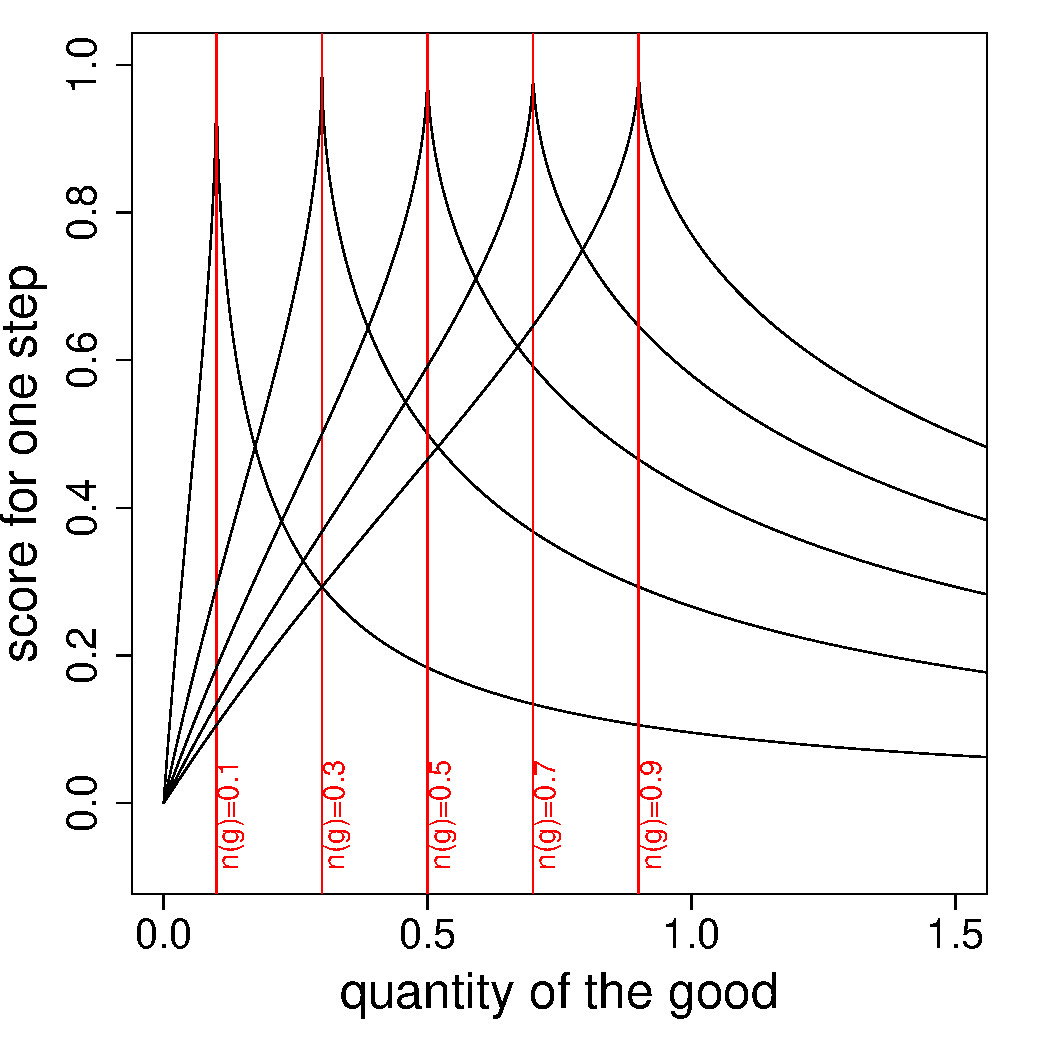
\includegraphics[width=7cm]{img/fitness.pdf}
%%	\end{center}
%%	\caption{The payoff depending on the quantity owned of a given good and the effective needs $n(g)$ for this good.}
%%	\label{fig:fit}
%%\end{figure}
%%Figure~\ref{fig:fit} depicts the score of an agent, for different need values of one good, with regards to the quantity of the good possessed by the agent. We can see that even if the need for a good is small (for instance when $n(g) = 0.01$) an agent can have a high score as soon as it manages to get a quantity close to the need. This ensures that an agent needs to have for each of the good a quantity equal to the need and that no agent could reach a better score just by getting the right quantity for a good with a high need.
%The complete score of an agent $i$ is termed $s^i$ and corresponds to the sum of the $s^i_j$. An agent will choose from whom the price vector should be copied among the agents that produce the same good and have the highest score. In practice, the worst (in terms of score) 20 percent of the agents producing the same good will copy the prices of the best twenty percent producing the same good. This selection process is detailed in algorithm~\ref{algo:selectionCulture}.
%
%
%\begin{algorithm}
%\caption{Selection Process}
%\label{algo:selectionCulture}
%	\begin{algorithmic}[1]
%	\scriptsize
%	\State	$ToGet = 0.2 \times \frac{\#Pop}{\#Good}$
%	\For{$g \in Good$}
%		\State	$ToReplace = \{\}$
%                \While{$\#ToReplace < ToGet$} 
%			\State $ j = SelectRand(Pop,g) $ \Comment{Select randomly an agent $j$ among the agents producing $g$}
%			\State $X \sim U([0,1])$ \Comment{Draw a random number from the uniform distribution between 0 and 1}
%			\If{$X>ComputeScore(j)$} \Comment{Select preferably the agents with the lowest scores}
%				\State $ToReplace = \{ToReplace,j\}$
%			\EndIf
%		\EndWhile
%
%                \While{$\#ToReplace > 0 $}
%			\State $ j = SelectRand(ToReplace) $ 
%			\State $ i = SelectRand(Pop,g) $  \Comment{Select randomly an agent $i$ among the agents producing $g$}
%			\State $X \sim U([0,1])$ 
%			\If{$ (X<ComputeScore(i))$} \Comment{Select preferably an agent $i$ with a high score}
%				\If {$ (ComputeScore(i)>ComputeScore(j))$} \Comment{Verify that agent $i$ has a higher score than agent $j$}
%					\State $CopyPrice(i,j)$
%					\State $ToReplace = ToReplace - i$
%				\EndIf
%			\EndIf
%
%		\EndWhile\
%	\EndFor
%\end{algorithmic}
%\end{algorithm}
%
%\paragraph{Trading} 
%During the trading phase the value associated to a good by an agent corresponds to the subjective price of the good for this agent. Briefly summarised, for each good that it does not produce, an agent will trade with the first partner that offers an acceptable trade, i.e. an agent that proposes a satisfiable ratio between the other good and the good produced by the agent. 
%
%In more details, the trading phase starts by the agent looking at a first random agent producing another good. 
%Let $o$ be an agent producing $g$ who proposes a trade and $r$ an agent producing $k$ that receives the proposition. As explained earlier, each has a quantity of good $Q^o$ and $Q^r$. On the one side, $o$ wants to exchange a quantity $w_g^o$ of the good $g$ for a quantity $w_k^o$ of the good $k$. On the other side, $r$ wants to exchange a quantity $w_g^r$ of the good $g$ for a quantity $w_k^r$. The tuples $W^o$ and $W^r$ describe the quantities of goods wanted by agent $o$ and $r$ for one trade proposition and are defined by:  
%
%\begin{equation}
%	 W^o=(w_g^o = v_g^o,w_k^o= \frac{v_k^o}{v_g^o}), \quad
%	 W^r=(w_k^r = v_k^r,w_g^r= \frac{v_g^r}{v_k^r}) 
%	 \label{eq:trade}
%\end{equation}
%
% Where $v_j^i$ are the estimated value of the good $j$ by the agent $i$ as defined earlier. 
%The requested quantity of the non produced good is simply the ratio between the estimated value of the good requested and the estimated value of the produced good.
%
%
%Once the quantities are defined, the agents declare that the trade is possible if :
%\begin{align}
%q_g^o >= w_g^o,\quad q_g^r <= w_g^o,\quad q_k^r >= w_k^o \label{eq:constraintQty}\\
%w_g^o>=(q_g^r+w_g^r),\quad w_k^o<=w_k^r,\quad w_g^o<=w_g^r \label{eq:constraintWill}
%\end{align}
%
%
%The conditions \ref{eq:constraintQty} ensure that both agents have enough goods in their inventory to realise the trade while the conditions \ref{eq:constraintWill} ensure that the quantities of goods fit the will of both agents.
%
%
%
%If a trade is possible, the two agents will exchange the agreed quantities. If the trade is not possible, the agent will continue to look at random partners for this good until either a partner is found or $TradeThreshold$ agents have been tried. At this point the agent will try to trade with agents producing another good. The process goes on until all goods have been tried. This trading process is described in algorithm~\ref{algo:trade}.
%
%\begin{algorithm}
%\caption{Trading Process for agent $o$}
%\label{algo:trade}
%	\begin{algorithmic}[1]
%	\scriptsize
%		\For{$j \in Goods \And j \neq produced^o $}
%			\State $tradeAttempt = 0$
%			\For{$r \in Pop \And produced^r = j \And tradeAttempt < TradeThreshold $}
%				\If{$acceptableTrade(W_o,W_r)$}
%					\State $trade(W_o,W_r)$
%				\Else
%					\State $tradeAttempt = tradeAttempt + 1$					
%				\EndIf
%			\EndFor
%		\EndFor
%\end{algorithmic}
%\end{algorithm}
%
%
%\paragraph{Innovation} In a trading environment it seems unlikely that a price will change radically to a very different value. Therefore, a new and more realistic mechanism is proposed. The innovation process, coined ``self referenced'', is still triggered with probability $\mu$ 
%but modifies the previous price by adding or subtracting a small amount taken randomly from a uniform  distribution between $0 .. \beta$.
%
%
%\paragraph{Expected outcome} Based on the set of implementations presented and given the equations (\ref{eq:score}) and (\ref{eq:trade}), it is expected that the prices will converge to value allowing each agent to obtain quantities of resources exactly equivalent to the needs. The best possible price of all good satisfies the equations :
%\begin{equation}
%	\begin{cases}
%		\frac{v^o_k}{v^o_g} = n_k \\
%		v^o_g = n_g 
%	\end{cases} =>v^o_k = n_k \times n_g, \quad \forall k \in Goods, \forall o \in Pop, g = produced^o, k \not= g 
%\end{equation}
%
%Which means that 
%
%\begin{equation}
%	\quad \forall j \in Goods, \forall i \in Pop \quad \tilde{V}^i = 
%	\begin{cases}
%		\tilde{v}^i_j = n_j & \text{if $ j=produced^i$}\\
%		 \tilde{v}^i_j = n_j \times n_{produced^i} & \text{else}
%	\end{cases}\label{eq:optimum}
%\end{equation}
%
%
%If such prices are reached, given the exchange rules defined in (\ref{eq:trade}) and the exchange constraints (\ref{eq:constraintQty}) and (\ref{eq:constraintWill}) all exchanges will be optimally achieved, leading to a total score $S$ for each agent of the population : 
%$$ S = \sum_{i=0}^{CulturalStep}  s^i(\tilde{Q}^i) \times ngoods $$ 
%where $\tilde{Q}^i$ is the optimal quantity vector, i.e. the one for which $s^i(\tilde{Q}^i) = s_{max}$. Remember that from equation~\ref{eq:score}, $s_{max}=1$.
%
%\subsection{Experimental setups}
%%In order to study the cultural transmission and the trading model two sets of implementation of the four processes of our model have been presented. Remember that during the definition of these two sets of implementation, two cultural transmission mechanisms have been defined () along with two innovation mechanisms (). Therefore, on top of exploring the results offered by the two set of implementations, it would be also interesting to understand which of the process is responsible for the variation in results. The four implementations proposed are summarized in the table~\ref{tab:exp}. Each couple of innovation/imitation mechanism form one setup that is labelled with one letter. Note that the ``neutral model" presented in section~\ref{sec:culturalTrans} corresponds to the setup A, and the trading model presented in section~\ref{sec:trade} corresponds to the setup D.
%%
%%\begin{table}[h]
%%	\centering
%%	\begin{tabular}{ll|cc}
%%				&	&\multicolumn{2}{c}{\textbf{Cultural transmission}} \\
%%		\multirow{2}[20]{*}{\rotatebox[origin=c]{90}{\textbf{Innovation}}}&  & Random & Success biased \\\hline  
%%		& \rule[-0.45cm]{0pt}{1cm} Unbounded 		&A & B \\
%%		& \rule[-0.45cm]{0pt}{1cm} Self Referenced	& C & D \\
%%	\end{tabular}
%%	\caption{Experimental Setup}
%%	\label{tab:exp}
%%\end{table}
%
%The neutral model is tested through 15 experimental setups. The first six experimental setups are using 1 good, two population sizes (250 and 500 agents) and three values of $\mu$ (0.004,0.016 and 0.064). The remaining experimental setups are using 500 agents, 3 number of goods (3,6 and 9) and three values of $\mu$ (0.004,0.016 and 0.064). For each setup, we have performed 100 runs of 10000 timestep each. The trading model is tested on an experimental setups using 3 goods, 500 agents and $\mu$ equal to 0.004. Again 100 runs of 10000 timesteps are performed. The experiments, as well as the parameters used to run those experiments, are \href{https://github.com/montanier/CMR-WSC-CoEvolutionTradeCulture}{available online} \cite{github_2015} for the Pandora simulator~\cite{rubiocampillo_2014}.
%
%%Finally, remember that in our experiment one has to take in account that agents modifies their prices or exchange their price only every $culturalStep$ steps. Between, twos such steps, the agent exchange goods given their own prices. Therefore we choose to run our simulation during 10000 step which correspond the 1000 time steps used by \cite{bentley_random_2004,mesoudi_random_2009}.
%
%%\begin{table}
%%\caption{Table of parameters}\label{tab:parameters}
%%	\scriptsize
%%\begin{center}
%%\begin{tabular}{@{}ll@{}}
%%\toprule
%%Parameter & Value \\
%%\midrule
%%Number of goods & $\{1,3,6,9\}$ \\
%%Number of agents & $\{250,500\}$ \\
%%Innovation probability ($\mu$) & $\{0.004,0.016,0.064\}$ \\
%%Innovation range ($\beta$) & 0.005\\
%%Cultural transmission probability & .001\\
%%CulturalStep &  10 \\
%%TradeThreshold & 100  \\
%%TimeSteps & 10000 \\
%%\bottomrule
%%\end{tabular}
%%\end{center}
%%\end{table}
%
%
%
%
%
%
}




\headerbox{Results}{name=res1,column=1,span=2,row=0}{
%\subsection{Neutral Model}

%We first analyse the result obtained in the ``neutral model" with one good. The figure~\ref{fig:allMutation} presents the results obtained for two population sizes $N$	 (250 and 500 agents) and $\mu$ varying through three values (0.004,0.016,0.064). The figure is a log-log plot of the average (across all the runs) of the distribution of variants obtained through all experiments. The y-axis shows the proportions of the variants of the prices used during the simulation, the x-axis shows how many variant achieves such proportions.
%
%\begin{figure}[!h]
%	\centering
%	\begin{tabular}{ c c}
%		 $N=250$ & $N=500$ \\
%		\includegraphics[width=6cm]{img/allmuRandMaxN250.pdf}&
%		\includegraphics[width=6cm]{img/allmuRandMaxN500.pdf}
%	\end{tabular}
%	\caption{Distribution of proportions depending on the $\mu$ parameter with 250 agents (left) and 500 agents (right). Each plot is the mean obtenaid for 100 runs.\label{fig:allMutation}}
%\end{figure}

%We observe that the lower the mutation rate, the closer to a line the result is. This line corresponds to the ``power law" distribution explained in section~\ref{sec:culturalTrans}, and is typical of the result obtained under the ``neutral hypothesis". In order to verify if the distribution is in fact a power-law, we follow the method proposed by~\cite{clauset2009powerlawdistributionsinempiricaldat} and the R implementation proposed by~\cite{gillespie_fitting_2015}. Briefly, two values are returned: a) the estimation of the $\alpha$ parameter of the power law equation $P(v)=C/v^\alpha $; b) a $p$-value testing the null-hypothesis that our data could have been generated from a power law distribution.
%
%%Within this method we fist fit a power law to the data of one simulation by estimating the parameters of the power law equation $P(v)=C/v^\alpha $. To estimate this, the method uses maximum likelihood estimator and Kolmogorof-Smirnov approach that gives use an estimated $\alpha$. The means of those $\alpha$ estimated for all simulations are summarized in the table~\ref{tab:mualpha}.
%%In a second step we check if the estimated parameters define effectively a power law that statistically describe the data obtained during the simulation. Using again Kolmogorof-Smirnov statistic, a number of fictive data points are generated based on the estimated power law. From this bootstrapping method we can then calculate a  
%
%The table~\ref{tab:mualpha} summarizes the results obtained on all setups. Each value shown in the table is the mean values of 100 simulations. We see that in almost every case the null hypothesis cannot be rejected, which means that indeed the repartition of the price follows a power law. The only exception is for $\mu$ equal to $0.064$, where the $p$-value is less than $0.05$. In this last case the null hypothesis is rejected, and we therefore assume that the distribution does not follow a power law.
%\begin{table}[H]
%	\caption{Mean $\alpha$ \& $sd$ are calculated on 100 runs for our results, and 5 runs for Bentley et. al. 2004. $pr$ is the percentage of run for which the $p$-value is less than 0.05, i.e. the percentage of runs for which we rejected the null-hypotheses stating that the distribution follow a power law.}
%	\centering
%	\scriptsize
%	\begin{tabular}{cc|ccc}
%		\multicolumn{2}{r}{}&\multicolumn{2}{c}{Our result}&\multicolumn{1}{c}{Bentley et. al. 2004}\\
%			N&$\mu$ & $\alpha$ ($sd$) & $p$-value ($sd$ - $pr$) &$\alpha$ ($sd$)\\\hline
%		250	&0.004&1.53 (0.03)&0.58 (0.24 - .01)&1.54 (0.02)\\
%			&0.016&1.57 (0.02)&0.35 (0.28 - .05)&1.57 (0.01)\\
%			&0.064&1.66 (0.01)&0.0 (0.00 - 1)&1.67 (0.01)\\\hline
%		500	&0.004&1.50 (0.02)&0.59 (0.28 - .02 )&1.53 (0.03)\\
%			&0.016&1.55 (0.03)&0.15 (0.17 - .10 )&1.61 (0.04)\\
%			&0.064&1.78 (0.08)&0.0 (0.00 - 1)&1.81 (0.10)\\
%	\end{tabular}
%	\label{tab:mualpha}
%\end{table}

%For comparison purposes the results obtained by~\cite{bentley_random_2004} (which tested the ``neutral hypothesis'' with the same methodology) are added in the last column of table~\ref{tab:mualpha}. It appears that these results are highly similar to ours. We note also that our results match the ones presented in~\cite{mesoudi_random_2009} where only one value of $\mu$ was tested ($\mu = 0.008$). However, it is difficult to know if the slight differences observed between our work and those previous studies are statistically significant as the two previous studies rely on only five runs for the computation of the mean of $\alpha$ (against 100 in our case).

%Nonetheless, for high values of $\mu$, previous works report that the distribution of variant follow a power law~\cite{bentley_random_2004}. This claim is based on the fact that the estimated $\alpha$ (estimation based on linear regression on the log-log curve) has a high correlation coefficient. Recent works have shown that the use of correlation coefficient should be avoided~\cite{clauset2009powerlawdistributionsinempiricaldat}. Following these recent findings, our results preclude us to assume that the distribution of variant when $\mu$ is up to $0.064$ follow a power law . 

%An additional series of experiments is done to analyse how the system reacts when multiple goods are present. The mean values of $\alpha$ and $p$-value have been analysed for 3 innovation rates (0.004, 0.016, 0.064), 4 number of goods (1, 3, 6, 9), and 250 agents. However, due to the simplicity of the results and the space restriction we only report the analysis of the results here. 
%\begin{table}[!h]
%	\centering
%	\begin{tabular}{l|llll}
%		Innovation rate &\multicolumn{4}{c}{Number of goods}\\
%		      & 1   & 3   &  6 & 9  \\\hline
%		0.004 &1.53 (0.03)  &1.53 (0.03)&1.53 (0.03)&1.53 (0.03) \\
%		0.016 &1.57 (0.02)  &1.57 (0.02)&1.56 (0.017)&1.57 (0.02) \\
%		0.064 &1.66 (0.01)  &1.66 (0.01)&1.66 (0.01)&1.66 (0.01) \\\hline
%	\end{tabular}
%	\caption{Mean $\alpha$ and standard deviation for all innovation rate and different  of goods. The $\alpha$ given here is the mean $\alpha$ among all goods taken separately and computed over 100 runs with 250 agents.}
%	\label{tab:multiGoods}
%\end{table}
%Visual analysis reveals that independently of the number of goods, the distributions obtained are exactly the same. Therefore it is no surprise that, for each innovation rate, the properties of the distribution of prices does not depend on the number of goods.

	\raggedcolumns
	\begin{multicols}{2}
\subsection*{Distribution of Cultural Variants}
We first compare the impact of different $CulturalTransmission$ mechanism on the distribution of frequencies of traits (the belief about the price of each goods). 
%In order to understand the effect of introducing trading mechanisms, we compare first the distribution of values obtained in the ``trading model'' against the values obtained in the ``neutral model''. The figure~\ref{fig:2setDi}.a) presents the results obtained from 100 runs for each model. All runs rely on the same experimental setup using 3 goods, 500 agents and $\mu$ equal to 0.004. In all following graph  a variant is one price of one given good. The distributions are first computed for each good independently and then averaged together.
\begin{figure}[H]
	\centering
%		a) & b)  \\
	%Frequencies distribution, where each points represent the mean for 100 runs, for: a) the neutral and the trading models.  b) the neutral model and the trading model without the trading innovation process. c) the trade model and the trade model without the trading innovation process.}
	\setlength{\columnseprule}{0pt}
	\begin{multicols}{2}
		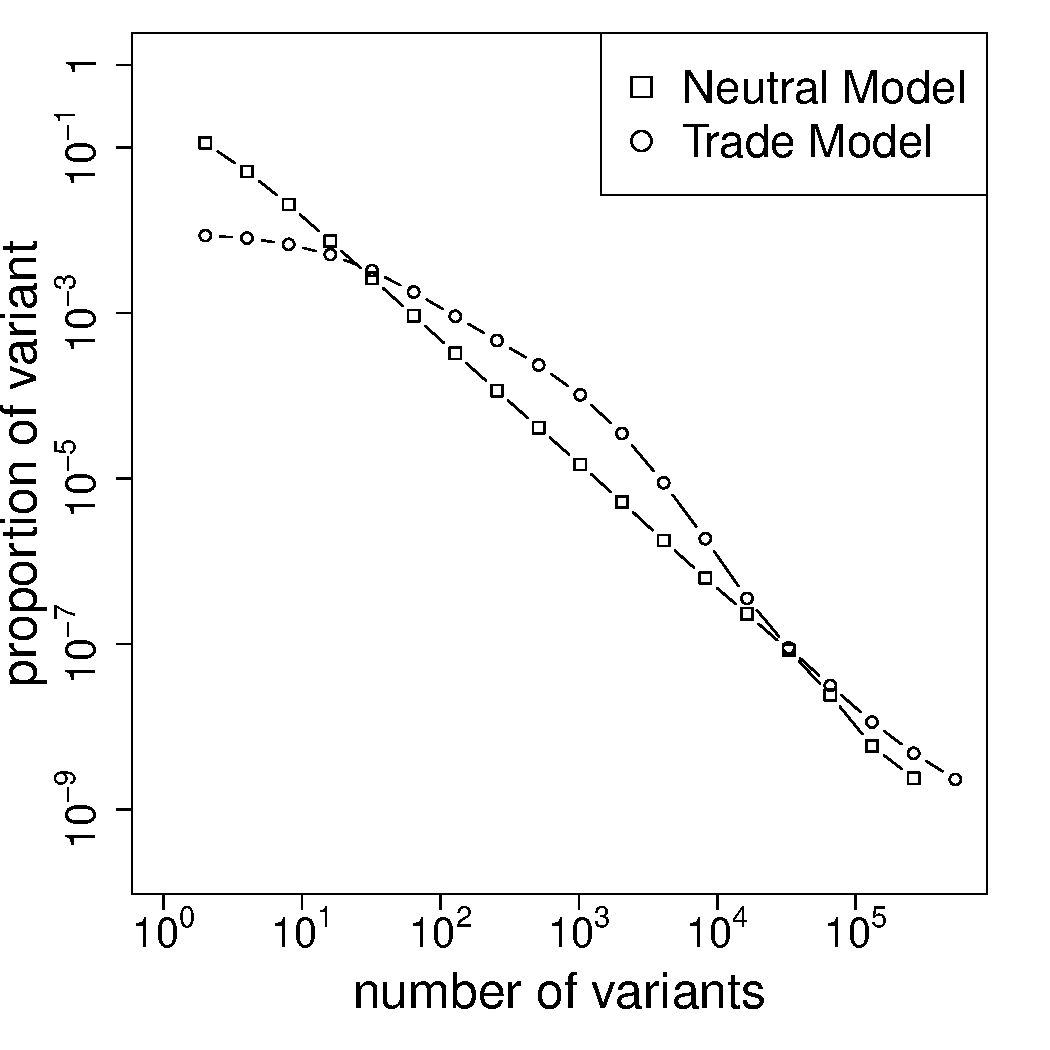
\includegraphics[width=5.2cm]{img/2SetupDistribA.pdf} 
	%	\includegraphics[width=5.2cm]{img/2SetupDistribB.pdf} &
	%	\includegraphics[width=5.2cm]{img/2SetupDistribD.pdf} \\
	%	a) & b) & c)  \\
		\caption{Comparaison of the distribution of frequencies between the neutral and the trade model.}
		\label{fig:2setDi}
	\end{multicols}
\end{figure}
\vspace{-.8cm}
Fig~\ref{fig:2setDi} shows that when $CulturalTransmission$ is neutral (agents randomly copy prices) the distribution follow the well know power law \cite{bentley_random_2004} but when transmission is not neutral but biased by the economical success of the agents, the power law disappear.
\subsection*{Economic Dynamics \& Equilibrium}

%The results obtained with the trade model are studied in more detail by investigating the ability of the population to find the price most suited for exchanges. This is done by first measuring the score of all agents in each of the two different models. The figure~\ref{fig:scoreEvol} uses again the results obtained from 100 runs for each model where all runs rely on the same experimental setup using 3 goods, 500 agents and $\mu$ equal to 0.004. The figure is showing, as boxplots, the score computed thanks to equation (\ref{eq:score}) for all agents of all runs. The y-axis shows the score computed and the x-axis shows the timesteps. The left plot shows the results obtained in the ``neutral model'' and the right plot shows the results obtained in the ``trading model''.


\begin{figure}[H]
	\centering
	\begin{tabular}{ c c}
		 Neutral Model & Trading Model \\
		 \includegraphics[width=5cm]{img/ScoreEvolutionForRandom-G3N500.pdf}
		 & 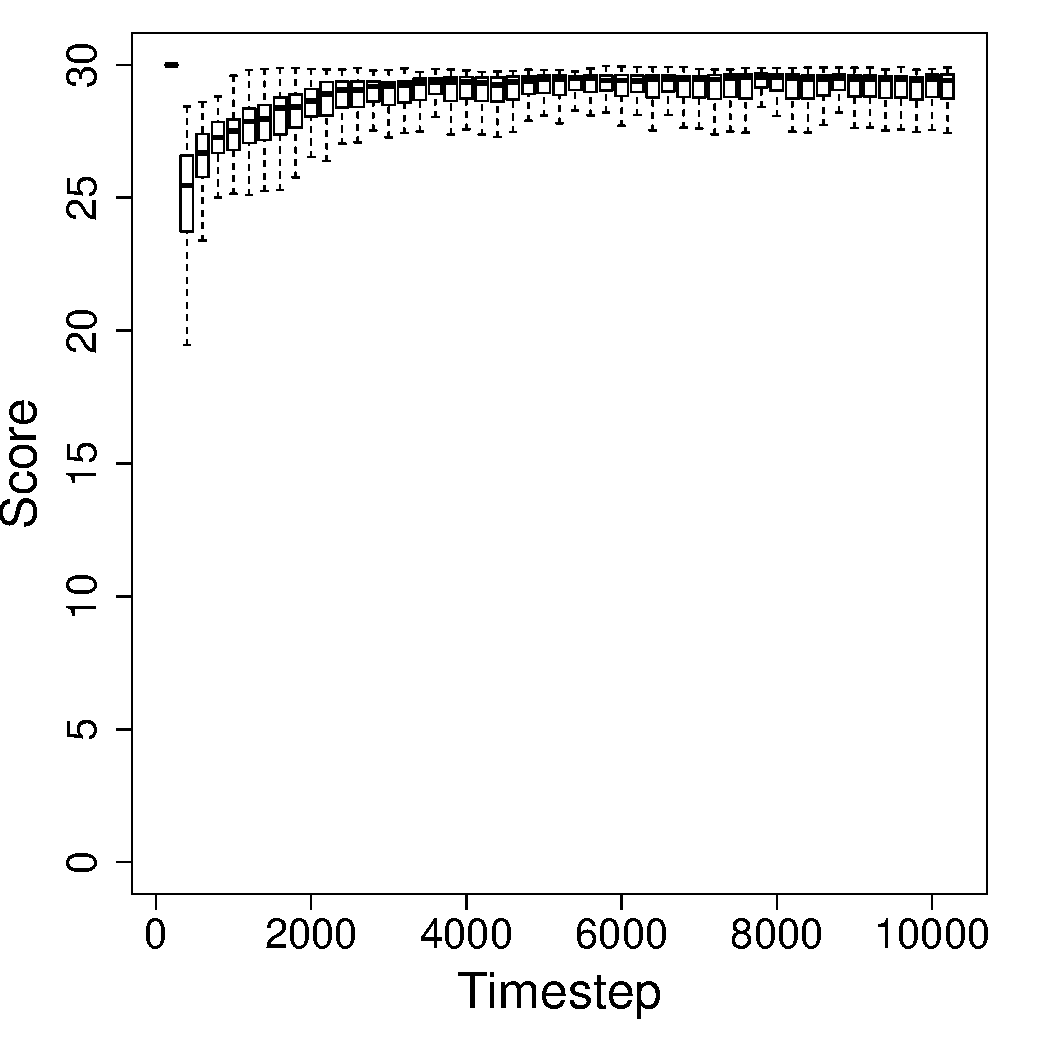
\includegraphics[width=5cm]{img/ScoreEvolutionForTrade-G3N500.pdf}

	\end{tabular}
	\caption{Evolution of the score within the two different models for two typical run with 500 agents and 3 goods evolving during 10000 timestep.}%%
	\label{fig:scoreEvol}
\end{figure}

As expected when $CulturalTransmission$ is random (ie, agents modify their belief about the prices randomly), the scores evolve randomly (fig~\ref{fig:scoreEvol}, left) wherease with a non random copy mechanism is used score increased toward the maximum score 
%In the setups A and C, the score evolves randomly. In the two other setups however the score is increasing. Moreover, we observe that the Self-referenced innovation process used in the setups C and D leads to higher convergences. Since only the ``biased transmission" takes the score into account it is normal that only this mechanism leads higher scores. The ``unbounded'' mechanism leads to lower convergences as it select prices randomly in the complete range available.

%As expected, the scores within the neutral model vary randomly. ``Trends'' may appear, where a bigger proportion of individuals adopt a better price that allow agents to reach better score (such as around iteration 8000), but such good score fall back as soon as another trend appears. However, with the trading model, the score of all the agents increase. As the selection mechanism allow them to know who has found better vectors of prices, they will progressively adopt prices vector that allow all of them to reach better scores. 
%
%The previous figure showed the capacity for the trading model to increase its score but did not analyse the exact prices used. As explained in the section~\ref{sec:trade} we expect that the trade \emph{cultural transmission} and \emph{innovation} processes will produce a convergence toward a set of price for each good that will allow agents to exchange optimally the good they produce with the other goods. To verify this assumption we analyse the prices reached during the simulations. These are presented in figure~\ref{fig:ratioEvol} for the 100 runs relying the experimental setup using 3 goods, 500 agents and $\mu$ equal to 0.004. For all runs, all agents and at each iteration we compute the difference between the price used by the agent $V_g$ and the optimal price $\tilde{V}_g$ (given by equation~\ref{eq:optimum}). The measures performed are presented as boxplots condensing the results for 100 runs.
%
\vfil
\columnbreak
%On figure~\ref{fig:2setDi}.a) it appears that the implementation of trade mechanisms leads to a distribution of prices departing from the neutral hypothesis. In more details, the frequencies distribution has a plateau of common prices (a number of prices share similar and high proportions), which shows that, when trade is taken into account, the most common variants are more diverse. 
%
%In order to investigate which mechanism influences this departure from the neutral model, additional investigations have been performed. Here is presented the results of the analysis on the effect of the \emph{innovation} process of the trade model. To conduct this analysis the \emph{innovation} process of the trade model has been replaced by the \emph{innovation} process of the neutral model. 100 runs have been performed with this model on the same experimental setup. The results obtained are compared to the neutral model in figure~\ref{fig:2setDi}.b) and to the trade model in figure~\ref{fig:2setDi}.c). 
%
%On figure~\ref{fig:2setDi}.b) it appears that the replacement of the innovation process leads to the creation of a distribution close to the one obtained with the neural model. On figure~\ref{fig:2setDi}.c) we observe a strong reduction in the size of the plateau and an important difference between the two distributions. This analysis highlights the importance of the \emph{innovation} process of the trading model in the distribution of prices. This mechanism, by preventing the creation of totally random new price, promotes the creation of few similar prices.
The raise of the score of the agents comes from the fact that the mechanism of $CulturalTransmission$ biased by the economic success of the agents, allows all the agents to quickly estimates prices that converge toward their optimal value (cf Fig~\ref{fig:ratioEvol}). Thus it allow them to make more efficient trade and increase their economic success (see also \cite{gintis_emergence_2006}).
\vspace{-.8cm}
\begin{figure}[H]
	\begin{multicols}{2}
	\begin{center}
		\includegraphics[width=5.5cm]{img/ClearingPriceDistanceEvolutionForTrade-G3N500.pdf}
	\end{center}
	\caption{
		Evolution of prices toward optimum prices.
		%Evolution of the mean of the difference between the estimated value $v^i_g$ and the optimal value $\tilde{v}^i_g$  for a good $g$ and an agent $i$. As the optimal value $\tilde{v}^i_g$ depends on which good is produced by $i$, the mean of the difference between the estimated price and the optimal one is computed between all the agents that produce the same good. The figure represents this mean computed at each timestep for each goods, for each groups of agents and for 100 runs in a setup with 500 agents and 3 goods. 
	}
	\label{fig:ratioEvol}
	\end{multicols}
\end{figure}
%We observe that prices are indeed converging to the optimal prices which means that the agents within the trading model are indeed improving their scores by reaching the optimal prices. Notably, a similar variation of prices was observed in the closely related economical model of~\cite{gintis_emergence_2006}. This variation of the prices to the optimum offers an additional conformation of the validity of the trading model. 
	\end{multicols}

}


\headerbox{Concluding Remarks}{name=conclusion,column=2,row=.42}{
	Integrating cultural and economical dynamics into a evolutionary framework is a good candidate to study such systems. It allows one to study precise mechanisms and to easily test and compare different model of such mechanisms.
	
	In futur work we hope to fruitfully apply that tools to bring different ways to propose, validate and interpret hypothesis about economics and cultural dynamics at work during the Roman Empire.

%This article has proposed a framework to simultaneously study cultural change and trade dynamics. The development of our framework was first aimed at simplicity which is achieved by the use of two vectors (quantity and value) and five processes (production, consumption, trade, cultural transmission and innovation). The second aim of the work conducted was to obtain a flexible framework which is possible since each of the processes can be implemented accordingly to the question studied. We have shown the validity of this approach by reproducing expected results on both the cultural and trade side. On the cultural transmission side we have shown that the implementation of a ``neutral model" leads to the expected observations on the variants of the vector value: a power law. When implementing trading mechanisms we observe the convergence of prices to the expected values and the improvement of the scores of the agents.

%The successful implementation of a trading model within our framework shows that trading models can be viewed as a particular implementation of the cultural evolutionary framework. This aspect which has not been studied before, opens a new line of thinking on the weight of trade mechanisms within cultural change. Notably, we have shown that the implementation of trade mechanisms leads to a distribution of prices departing from the neutral hypothesis, which is the reference in the study of cultural changes. Within the trading model, the frequency distribution has a plateau of common prices (a number of prices share similar and high proportion), which shows that, when trade is taken into account, the most common variants are more diverse. Interestingly, we have not find references pointing at the ability of trade mechanisms to keep a relatively large diversity in the frequency distribution. We suspect that this is mainly because it is not common to compare results of trading models to other cultural evolution models. It would therefore be interesting to compare the frequency distributions obtained by our model and the ones observed in current or past economies. On the side of cultural transmission, the results obtained can also be compared to the ones obtained when prestige biased cultural transmission is used. The idea behind this last comparison, is that trade could be interpreted as a particular prestige biased cultural transmission and therefore be fully integrated within the cultural evolutionary frameworks.

%%% proposition extention authors
%    For example, what happens if there are two populations with distinct tastes (and separate replicators)? How reactive are prices to shifts in production/needs? (innovation will become useful to remedy the lack of genetic diversity needed to deal with shifts)
%    If replication and imitation were to happen on a social network rather than at random, how much slower would the the correct prices emerge?
%    Would the plateau of common prices disappear if you were to add single-crossover replication of the value vector in the cultural transmission algorithm?

%In future works more realistic scenarios can be studied in the same framework. Multiple implementations of the production mechanism can be studied so as to increase the number of goods per agent and include factors such as the meteorology or the various type of goods. Moreover, the introduction of the distinction between ``vital'' and ``common'' goods will be useful for the creation of models studying in further details the interaction between trade and cultural transmission. 
%
%Additionally, more complex dynamics can be looked for. The trading mechanism can be naturally implemented in different ways, each reflecting a specific theory, and thus allowing their comparisons. The cultural transmission mechanism also can be modified by including for example a crossover between the cultural trait of multiple agents. The trade network (which in this work can be interpreted as fully connected) can also be modified to study the effect of slow connections or the rupture of certain connections. The agent themselves could become more complex and be endowed with the ability to learn behaviours which would again produce more realistic simulations. Moreover, various populations can be envisioned, each with their distinctive characteristics regarding cultural transmission and trade. 
%
%Finally, in terms of analysis of the results, multiple factor could be taken into account. The rapidity of the fluctuation of prices is a good starting point for the establishment of economical studies. For the study of a population of agent in general, it can be interesting to analyse the number of agents active and the composition of the population.
}


\headerbox{References}{name=references,column=2,below=conclusion}{
	\scriptsize

	\renewcommand{\refname}{\vspace{-0.8em}}
	\bibliographystyle{unsrt}
	\bibliography{biblio}
}
\headerbox{Acknowledgements}{name=acknowledgements,column=2,below=references}{
Funding for this work was provided by the ERC Advanced Grant EPNet (340828) and the SimulPast Consolider Ingenio project (CSD2010-00034) of the former Ministry for Science and Innovation of the Spanish Government. 
	\begin{center}
		\coloremph{http://http://www.roman-ep.net/epnet/}
	\end{center}

} 

\end{poster}

\end{document}

